\chapter{Attaque SSLstrip 2}

\label{sec:sslstrip2}

\begin{figure}[H]
  \caption{Attaque SSLstrip 2 (diagramme Dia)}
  \fbox{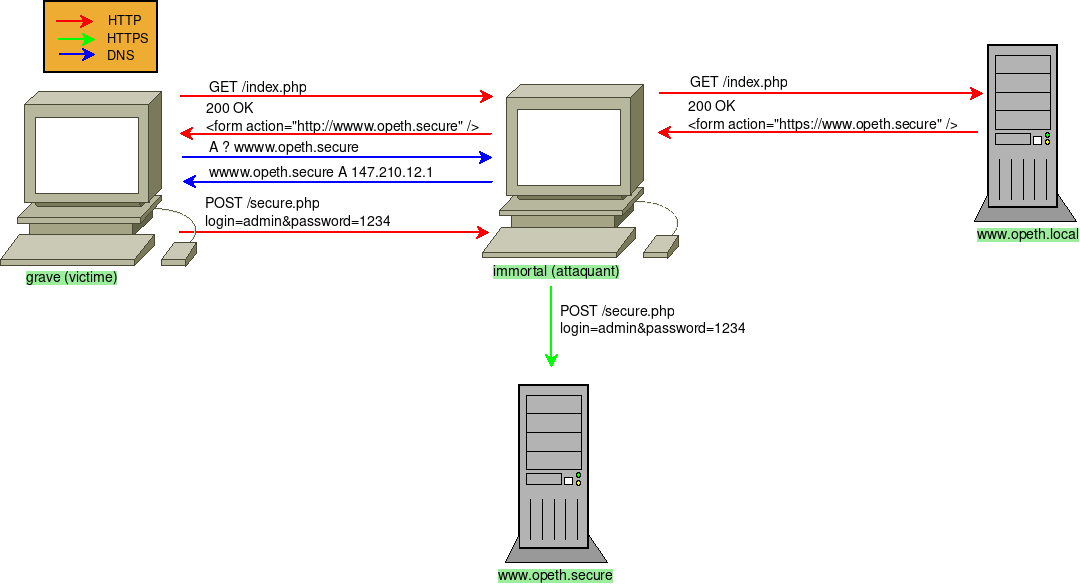
\includegraphics[width=\textwidth]{../medias/sslstrip2/attack.png}}
\end{figure}

Comme vu précédemment, une contre-mesure a été mise en place afin de déclarer aux clients d'un serveur qu'ils doivent utiliser une connexion sécurisée en HTTPS pour leur futures connexions avec celui-ci. Vous pouvez vous reporter à la section \hyperref[sec:hsts]{Contremesures} pour plus de précision.

Notre but est donc de contourner le HSTS en réutilisant l'attaque SSLStrip. Malheureusement, on ne peut pas la réutiliser directement car le navigateur a gardé en mémoire que toutes connexions sur cette page doivent se faire en HTTPS.

\section{Description de l'attaque}
Cette extension de SSLStrip a été pensée par LeonardoNve en 2014. Elle permet donc de passer au travers l'une des nouvelles contre-mesures mise en place sur les navigateurs. En effet, si l'attaquant se place en homme du milieu, il va pouvoir intercepter le trafic entre le client et le serveur afin de le faire réagir comme suit.

Lorsque le client va se connecter au serveur sur une page HTTP, l'attaquant va modifier cette page en remplaçant tous les liens HTTPS en HTTP mais aussi en changeant le nom de domaine. Changer le nom de domaine changera le comportement du navigateur. En effet, comme le navigateur ne connaît pas ce nom de domaine, il n'enverra pas d'exception liée à HSTS.

Voici un exemple :

Si le lien est \path{https://www.domain.secure}, on peut le remplacer par \path{http://wwww.domain.secure}.

Il faut noter que l'on enlève le \verb+s+ de \verb+https+ et que l'on remplace \verb+www+ par \verb+wwww+ ce qui change bien le nom de domaine.

Ainsi, l'attaquant fait croire au navigateur que cette requête est légitime et que \path{wwww.domain.secure} correspond au serveur distant. La connexion sera donc en HTTP et donc en clair.

\section{Notre attaque}

Tout d'abord, afin de pouvoir mettre en place l'attaque, il nous faut configurer l'environnement. Rappelons que l'attaquant est déjà positionné en homme du milieu, et que nous avons choisi de mettre sa machine dans le même réseau que la machine victime. Comme pour l'attaque précédente, nous utilisons l'outil \verb+qemunet+ développé par l'Inria qui nous permet de créer un environnement minimaliste et léger. Il nous faut donc vous expliquer sa mise en place.

\subsection{Mise en place de l'environnement}

\subsubsection{Configuration de la machine serveur - opeth}

Pour cette attaque, nous avons besoin d'un serveur DNS, installé sur la machine \textbf{opeth}. Pour cela, nous utilisons l'outil DNSMASQ. Le fichier \path{sslstrip2/opeth/dnsmasq.conf} spécifie notre nom de domaine et les actions relatives à la résolution du nom de domaine.

\inputminted[bgcolor=lbcolor, breaklines]{shell}{../sslstrip2/opeth/dnsmasq.conf}

On obtient donc le script de lancement suivant qui charge toutes les configurations et associe l'adresse IP de opeth aux noms de domaines suivants :

\begin{itemize}
\item \path{www.opeth.local} lorsque l'on accède en HTTP à la page ;
\item \path{www.opeth.secure} lorsque l'on accède en HTTPS.
\end{itemize}

\inputminted[bgcolor=lbcolor, breaklines]{shell}{../sslstrip2/opeth/start.sh}

\subsubsection{Configuration de la machine attaquante - immortal}


Cette machine utilise également DNSMASQ afin d'usurper les requêtes DNS de grave.

Comme précisé dans la description de l'attaque, nous avons besoin d'un nom de domaine supplémentaire afin de rediriger les requêtes DNS dessus. Ce nom de domaine est \path{wwww.opeth.secure}. On n'a donc besoin d'une règle dans la table PREROUTING de iptables afin de rediriger les paquets sur son propre serveur lorsque l'attaque à lieu.

Voici le contenu du fichier \path{/mnt/host/attack.sh} pour cette attaque :

\inputminted[bgcolor=lbcolor, breaklines]{shell}{../sslstrip2/immortal/attack.sh}

Nous commençons par rediriger les requêtes HTTP (port 80) sur le port de notre proxy (port 4242), puis les requêtes DNS sont redirigées vers le serveur DNS de l'attaquant.

\subsection{Démonstration}

Après ces présentations de mise en place, nous pouvons vous montrer le fonctionnement de l'attaque via une démonstration. Pour lancer l'environnement de test, il faut utiliser la commande suivante (on aura récupéré préalablement le dépôt \textbf{qemunet}) :

\begin{minted}{bash}
  ./qemunet/qemunet.sh -x -S sslstrip2
\end{minted}

Maintenant, nous avons les trois machines de lancées. Les login et mot de passe sont :

\begin{itemize}
\item grave : toto - toto
\item immortal : root - rien
\item opeth : root - rien
\end{itemize}

\subsubsection{Étape 1 : Avant l'attaque}

Avant de vous montrer ce qu'il se passe lors de l'attaque, nous devons vous montrer l'état initial.

Lorsque l'attaque n'est pas lancée, nous pouvons voir sur la machine grave que la communication se passe sans problèmes et que la requête POST passe bien en HTTPS; immortal est donc incapable de voir les identifiants envoyés :

\begin{figure}[H]
  \caption{Attaque SSLstrip2 (avant l'attaque)}
  \fbox{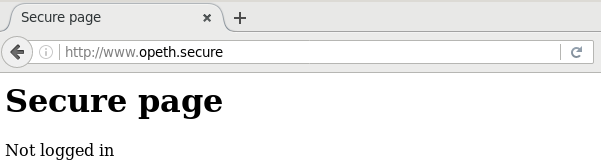
\includegraphics[width=\textwidth]{../medias/sslstrip2/screen1.png}}
\end{figure}

L'encadré rouge ci-dessous montre bien que le POST est effectué en HTTPS, sur le domaine \path{www.opeth.secure}. Lorsque nous affichons le code source de la page, nous obtenons :

\begin{figure}[H]
  \caption{Code source de la page (avant l'attaque)}
  \fbox{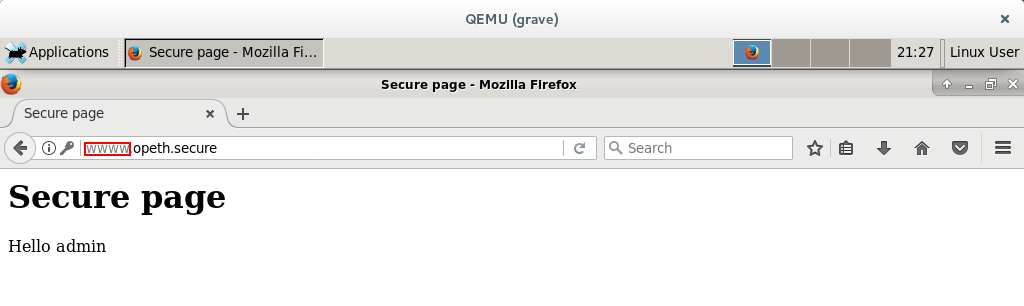
\includegraphics[width=\textwidth]{../medias/sslstrip2/screen2.png}}
\end{figure}

Nous arrivons alors sur le domaine \path{www.opeth.secure} en HTTPS : immortal n'a pas pût voir nos échanges sur cette page sécurisée comme le montre la figure ci-dessous.

\begin{figure}[H]
  \caption{La connexion se fait bien en https}
  \fbox{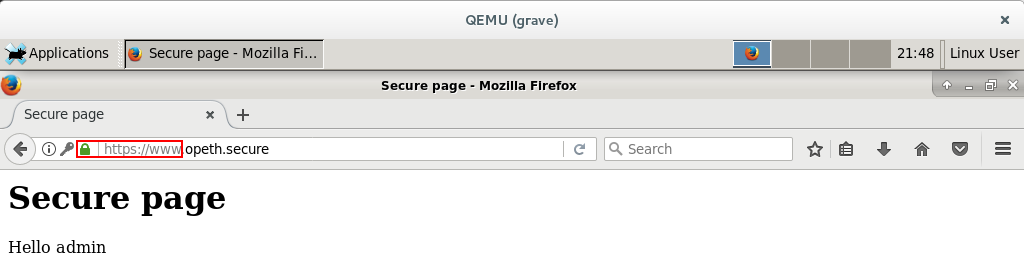
\includegraphics[width=\textwidth]{../medias/sslstrip2/screen3.png}}
\end{figure}

\subsubsection{Étape 2 : lancement de l'attaque}

Comme expliqué précédemment, pour lancer l'attaque, il faut exécuter le fichier \path{/mnt/host/attack.sh} depuis immortal dont on a déjà expliqué son comportement.

Nous pouvons maintenant lancer l'attaque depuis la machine immortal :


\begin{figure}[H]
  \caption{Lancement de l'attaque}
  \fbox{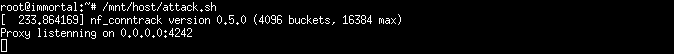
\includegraphics[width=\textwidth]{../medias/sslstrip2/screen4.png}}
\end{figure}

\paragraph{Explication du code \\}

Le code du proxy est dans le dossier de la machine immortal, le fichier \path{sslstrip2.py}.

\subparagraph{Réception des requêtes \\}

Lors de la réception de requêtes, il s'agit de savoir si l'on doit :

\begin{itemize}
\item fermer la connexion (le client ou le serveur a fermé la connexion)
\item établir une connexion en HTTPS, dans le cas où le client va sur le domaine \path{wwww.opeth.secure}
  \item établir une connexion HTTP, dans le cas où le client demande la page du domaine \path{www.opeth.local}
\end{itemize}

La fonction traitant les différentes requêtes est celle-ci :

\begin{minted}{python}
def __recv(self, csock):
        fw_sock = self.__csockets[csock]
        data = csock.recv(BUFFER_SIZE)
        if len(data) == 0:
            self.__close_conn(csock)
            self.__close_conn(fw_sock)
        else:
            print(data)

            if fw_sock is None:
                m = re.search(b'Host: (\S+)', data)
                if m is not None and m.group(1) == FAKE_HOST:
                    re.sub(b'Host: (\S+)',
                           b'Host: ' + bytes(FORWARD_HOST_HSTS), data)
                    self.__new_https_conn(csock)
                else:
                    self.__new_http_conn(csock)
                fw_sock = self.__csockets[csock]
            data = self.__replace_https_to_http(data)
            data = self.__replace_host(data)
            data = self.__replace_content_length(data)
            fw_sock.send(data)
\end{minted}

À la fin, on transforme tous les liens HTTPS trouvés en HTTP en remplaçant le nom de domaine \path{www.opeth.secure} par le faux nom de domaine \path{wwww.opeth.secure}, on met l'entête Host vers le bon domaine et on recalcule la taille de la requête (entête Content-Lenght)

\subparagraph{Transformation des liens \\}

Dans cette fonction, nous utilisons une expression régulière afin de remplacer tous les liens \path{https://www.opeth.secure} en \path{http://wwww.opeth.secure}.

\begin{minted}{python}
def __replace_https_to_http(self, data):
    return re.sub(b'https://' + bytes(FORWARD_HOST_HSTS),
                  b'http://' + bytes(FAKE_HOST), data)
\end{minted}

\subparagraph{Modification de l'entête Host}

Lorsque la victime est redirigée vers un lien \path{http://wwww.opeth.secure}, l'entête Host de ses requêtes sera erronée. Cette fonction modifie cette entête pour que le serveur puisse recevoir un Host correct.

\begin{minted}{python}
def __replace_host(self, data):
    return re.sub(b'Host: ' + bytes(FAKE_HOST),
                  b'Host: ' + bytes(FORWARD_HOST_HSTS), data)
\end{minted}


\subparagraph{Recalcul de l'entête Content-Length}

La taille de la requête étant modifiée par le proxy, celui-ci doit recalculer l'entête Content-Length en se basant sur la chaîne "{\textbackslash}r{\textbackslash}n{\textbackslash}r{\textbackslash}n" signalant la fin des entêtes dans le protocole HTTP.

\begin{minted}{python}
def __replace_content_length(self, data):
    try:
        idx = data.index(b"\r\n\r\n")
        length = len(data) - idx - 4
        return re.sub(b'Content-Length: (\d+)',
                      b'Content-Length: %d' % length, data, 1)
    except:
        return data
\end{minted}

\subsubsection{Étape 3 : Pendant l'attaque}

Lorsque l'attaque est lancée, on peut voir que le lien sensible \path{https://www.opeth.secure} est remplacé par \path{http://wwww.opeth.secure}.
La machine immortal est donc capable d'intercepter les échanges réalisés sur le domaine \path{www.opeth.secure}.

Dans cette image, on voit dans l'encadré rouge, que le lien \path{https://} a bien été remplacé par un lien non sécurisé \path{http://} :

\begin{figure}[H]
  \caption{Le 's' de "https" a disparu}
  \fbox{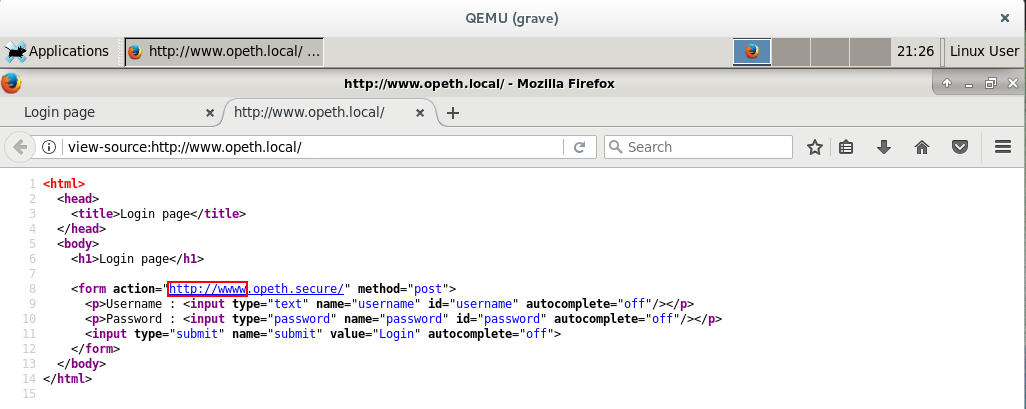
\includegraphics[width=\textwidth]{../medias/sslstrip2/screen5.png}}
\end{figure}

Nous constatons que nous arrivons sur la page secure.php en HTTP : notre navigation n'est pas sécurisée !

\begin{figure}[H]
  \caption{Le client visite une page sécurisée en http}
  \fbox{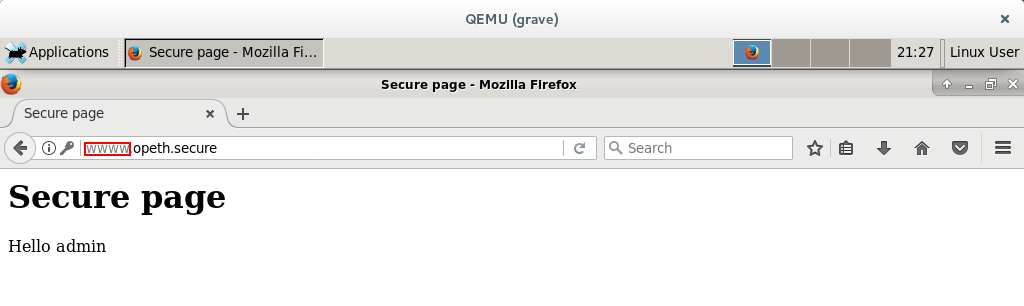
\includegraphics[width=\textwidth]{../medias/sslstrip2/screen6.png}}
\end{figure}

La machine immortal a été capable de capturer non seulement les identifiants du formulaire, mais également le cookie de session :

\begin{figure}[H]
  \caption{L'attaquant récupère toutes les informations sensibles}
  \fbox{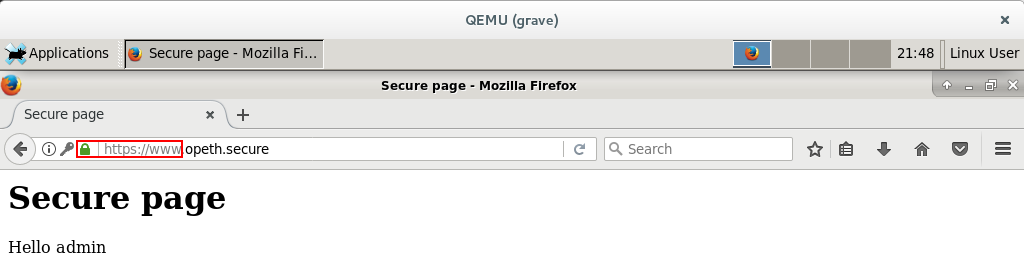
\includegraphics[width=\textwidth]{../medias/sslstrip2/screen7.png}}
\end{figure}

Le script complet de l'attaque peut être consulté à l'annexe \ref{appendix:sslstrip2}.
